\documentclass[10pt]{article}
\usepackage{amsmath}
\usepackage{mathtools}
\DeclarePairedDelimiter{\abs}{\lvert}{\rvert}
\usepackage[hidelinks]{hyperref}
\usepackage{amssymb}
\usepackage{tikz}
\usepackage{caption}
\usepackage{graphicx}
\usepackage[T1]{fontenc}
\graphicspath{{.}}
\usepackage{listings}
\usepackage{verbatim}
\lstset{
language=[LaTeX]TeX,
backgroundcolor=\color{gray!25},
basicstyle=\ttfamily,
columns=flexible,
breaklines=true
}
\captionsetup{labelsep=space,justification=justified,singlelinecheck=off}
\reversemarginpar
\usepackage[paper=a4paper,
            %includefoot, % Uncomment to put page number above margin
            marginparwidth=10mm,      % Length of section titles
            marginparsep=0.8mm,       % Space between titles and text
            margin=11mm,              % 25mm margins
            includemp]{geometry}

\begin{document}
\section*{}
\begin{flushleft}
CSCI 5502 - Data Mining - Homework 4\\
Name: Krishna Chaitanya Sripada\\
Student ID: 104375417\\
Honor Pledge: On my honor, as a University of Colorado at Boulder student, I have neither given nor received unauthorized assistance on this work.
\end{flushleft}
\section*{Ans 1}
\begin{flushleft}
(a) The number of candidate 3-itemsets in total are 22 i.e., L1 has 2, L2 has 2, L3 has 3, L4 has 3, L5 has 1, L6 has 2, L7 has 2, L8 has 1, L9 has 3, L11 has 2 and L12 has 1. So a total of 22 candidate 3-itemsets.\\
\vspace{0.5em}
Without using hash tree, the number of candidate 3-itemsets we need to check for each transaction is ${k \choose 3}$ where `k' is the number of items. Here k = \{1,2,3,4,5,6,7,8,9\}. Therefore, the number of candidate 3-itemsets = ${9 \choose 3} = 84$.\\
\vspace{1em}
(b) The list of candidate 3-itemsets for the items \{1,3,4,6,8\} are \{1,3,4\}, \{1,3,6\}, \{1,3,8\}, \{1,4,6\}, \{1,4,8\}, \{1,6,8\}, \{3,4,6\}, \{3,4,8\}, \{3,6,8\}, \{4,6,8\}. The hash tree leaf nodes that need to visited are : L1, L5, L9 and L12 i.e, for transactions with prefix \{1,3\}, the L5 node is visited. For transactions with prefix \{1,4\}, the L1 node is visited. The transactions with prefix \{1,6\}, the L5 node is visited. For transactions with prefix \{3,4\}, the L9 node is visited. For transactions with prefix \{3,6\}, the L12 node is visited and finally for transactions with prefix \{4,6\}, the L5 node is visited.\\
\vspace{1em}
(c) The candidate item sets contained in the transaction \{1,3,4,6,8\} are \{1,6,8\} and \{3,4,6\}.
\end{flushleft}
\section*{Ans 2}
\begin{flushleft}
(a) Rule $v \notin S$ is monotonic but not antimonotonic. \\
\textbf{Antimonotonic Example:} Let v = 4 and S = \{1,2,4\}. Now itemset S violates the rule $v \notin S$. Let $S^{'}$ be the superset= \{1,2,4,5\}. Here the superset $S^{'}$ also violates the rule $v \notin S$. Thus the rule is antimonotonic.\\
\vspace{0.5em}
\textbf{Not Monotonic Example:} Let v = 5 and S = \{1,2,4\}. Now itemset S satisfies the rule $v \notin S$. Let $S^{'}$ be the superset= \{1,2,4,5\}. Here the superset $S^{'}$ does not satisfy the rule $v \notin S$. Thus the rule is not monotonic.\\
\vspace{0.5em}
Therefore, the rule $v \notin S$ is monotonic but not antimonotonic is \textbf{false}.\\
\vspace{1em}
(b) Rule $V \subset S$ is monotonic but not antimonotonic.\\
\textbf{Monotonic Example:} Let V = \{2,3\} and S = \{2,3,6,7\}. Now itemset S satisfies the rule $V \subset S$. Let $S^{'}$ be the superset = \{2,3,6,7,8,9\} also satisfies the rule. Thus the rule is monotonic.\\
\vspace{0.5em}
\textbf{Not Antimonotonic Example:} Let V = \{2,3\} and S = \{4,5,6,7\}. Now itemset S violates the rule $V \subset S$. Let $S^{'}$ be the superset = \{4,5,6,7,2,3\}. Here the superset $S^{'}$ does not violate the rule. Thus the rule is not antimonotonic.\\
\vspace{0.5em}
Therefore, the rule $V \subset S$ is monotonic but not antimonotonic is \textbf{true}.\\
\vspace{1em}
(c) Rule $avg(S) \geq v$ can be converted into a monotonic rule.\\
\textbf{Monotonic Example:} Let v = 25 and S = \{25,50,75,100,125,150\} where the items in the itemset S are ordered in an ascending order, the $avg(S)$ = 87.5 satisfies the rule. Let $S^{'}$ be the superset = \{25,50,75,100,125,150,175,200\} where the items in the itemset $S^{'}$ are also ordered in an ascending order, the $avg(S)$ = 112.5 also satisfies the rule.\\
\vspace{0.5em}
Therefore, the rule $avg(S) \geq v$ can be converted into a monotonic rule is \textbf{true}.\\
\end{flushleft}
\section*{Ans 3}
\begin{flushleft}
(a) Given ``Seat Belt'' is the class label. Now using information gain as the attribute selection measure, we calculate the following:\\
\vspace{0.5em}
Expected information needed to classify a tuple in our dataset is,\\
\hspace{2em} $Info(D) = - \frac{8}{12} \log_2 (\frac{8}{12}) - \frac{4}{12} \log_2(\frac{4}{12})$\\
\vspace{0.5em}
\hspace{6.1em} $ = 0.39 + 0.528 = 0.918$ bits\\
\vspace{0.5em}
Now, we need to compute the expected information requirement for each attribute. \\
\vspace{0.5em}
(i) The first attribute is ``Weather Condition''. The expected information needed to classify a tuple in the dataset if the tuples are partitioned according to Weather Condition is, \\
\vspace{0.5em}
In ``Bad'' category, there are 3 yes tuples and 2 no tuples and in the ``Good'' category, there are 5 yes tuples and 2 no tuples. Therefore, \\
\vspace{3em}
\hspace{2em} $Info_{WC}(D) = \frac{5}{12} * ( - \frac{3}{5} \log_2 \frac{3}{5} - \frac{2}{5} \log_2 \frac{2}{5}) + \frac{7}{12} * (- \frac{5}{7} \log_2 \frac{5}{7} - \frac{2}{7} \log_2 \frac{2}{7})$\\
\vspace{0.5em}
\hspace{7.6em} $ = 0.404 + 0.502 = 0.906$ bits\\
\vspace{0.5em}
Hence, the gain in information for such a partitioning would be, \\
\vspace{0.5em}
\hspace{2em} $Gain(Weather Condition) = Info(D) - Info_{WC}(D) = 0.918 - 0.906 = 0.012$ bits.\\
\vspace{1em}
(ii) The second attribute is ``Driver's Condition''. The expected information needed to classify a tuple in the dataset if the tuples are partitioned according to Driver's Condition is,\\
\vspace{0.5em}
In ``Sober'' category, there are 5 yes tuples and 2 no tuples and in ``Alcohol-impaired'' category, there are 3 yes tuples and 2 no tuples. Therefore, \\
\vspace{0.5em}
\hspace{2em} $Info_{DC}(D) = \frac{7}{12} * ( - \frac{5}{7} \log_2 \frac{5}{7} - \frac{2}{7} \log_2 \frac{2}{7}) + \frac{5}{12} * (- \frac{3}{5} \log_2 \frac{3}{5} - \frac{2}{5} \log_2 \frac{2}{5})$\\
\vspace{0.5em}
\hspace{7.5em} $= 0.502 + 0.404 = 0.906$ bits\\
\vspace{0.5em}
Hence, the gain in information for such a partitioning would be, \\
\vspace{0.5em}
\hspace{2em} $Gain(Driver's Condition) = Info(D) - Info_{DC}(D) = 0.918 - 0.906 = 0.012$ bits.\\
\vspace{1em}
(iii) The third attribute is ``Traffic Violation''. The expected information needed to classify a tuple in the dataset if the tuples are partitioned according to Traffic violation is,\\
\vspace{0.5em}
In ``None'' category, there are 2 yes tuples and 1 no tuple. In ``Disobey stop sign'' category, there are 3 yes tuples and 0 no tuples. In ``Exceed speed limit'', there are 2 yes tuples and 1 no tuple. In ``Disobey traffic signal'' category, there are 1 yes tuple and 2 no tuples.\\
\vspace{0.5em}
\hspace{2em} $Info_{TV}(D) = \frac{3}{12} * ( - \frac{2}{3} \log_2 \frac{2}{3} - \frac{1}{3} \log_2 \frac{1}{3}) + \frac{3}{12} * (- \frac{3}{3} \log_2 \frac{3}{3}) + \frac{3}{12} * (- \frac{2}{3} \log_2 \frac{2}{3} - \frac{1}{3} \log_2 \frac{1}{3}) + \frac{3}{12} * (- \frac{1}{3} \log_2 \frac{1}{3} - \frac{2}{3} \log_2 \frac{2}{3})$\\
\vspace{0.5em}
\hspace{5em} $= 0.229 + 0 + 0.229 + 0.229 = 0.687$ bits\\ 
\vspace{0.5em}
Hence, the gain in information for such a partitioning would be, \\
\vspace{0.5em}
\hspace{2em} $Gain(Traffic Violation) = Info(D) - Info_{TV}(D) = 0.918 - 0.687 = 0.231$ bits.\\
\vspace{1em}
(iv) The fourth attribute is ``Crash Severity''. The expected information needed to classify a tuple in the dataset if the tuples are partitioned according to Crash Severity is,\\
\vspace{0.5em}
In ``Minor'' category, there are 4 yes tuples and 0 no tuples. In ``Major'' category, there are 4 yes tuples and 4 no tuples.\\
\vspace{0.5em}
\hspace{2em} $Info_{CS}(D) = \frac{4}{12} * (- \frac{4}{4} \log_2 \frac{4}{4}) + \frac{8}{12} * (- \frac{4}{8} \log_2 \frac{4}{8} - \frac{4}{8} \log_2 \frac{4}{8})$\\
\vspace{0.5em}
\hspace{7.3em} $ = 0 + 0.666 = 0.666$ bits\\
\vspace{0.5em}
Hence, the gain in information for such a partitioning would be, \\
\vspace{0.5em}
\hspace{2em} $Gain(Crash Severity) = Info(D) - Info_{CS}(D) = 0.918 - 0.666 = 0.251$ bits.\\
\vspace{1em}
Because ``Crash Severity'' has the highest information gain among the attributes, it is selected as the splitting attribute.\\
\vspace{1em}
\begin{figure}[!htb]
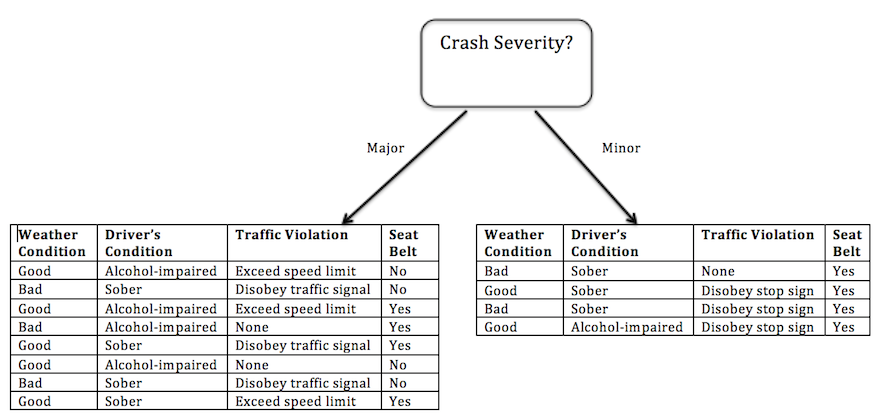
\includegraphics{dt1.png}
\caption{:First Level Decision Tree}
\end{figure}
\vspace{1em}
(b) Since we are using gain ratio as the attribute selection measure, the following is the information calculated:\\
(i) For the first attribute ``Weather Condition'' splits the data into two partitions ``Bad'' and ``Good'' containing 5 and 7 tuples respectively, therefore, \\
\vspace{0.5em}
\hspace{2em} $SplitInfo_{WC}(D) = - \frac{5}{12} \log_2 \frac{5}{12} - \frac{7}{12} \log_2 \frac{7}{12}$\\
\vspace{0.5em}
\hspace{9.8em} $ = 0.526 + 0.453 = 0.97$\\
\vspace{0.5em}
\hspace{2em} $GainRatio(Weather Condition) = \frac{0.012}{0.97} = 0.012$\\
\vspace{1em}
(ii) For the second attribute ``Driver's Condition'' splits the data into two partitions ``Sober'' and ``Alcohol-impaired'' containing 7 and 5 tuples respectively, therefore, \\
\vspace{0.5em}
\hspace{2em} $SplitInfo_{DC}(D) = - \frac{7}{12} \log_2 \frac{7}{12} - \frac{5}{12} \log_2 \frac{5}{12}$\\
\vspace{0.5em}
\hspace{9.7em} $ = 0.453 + 0.526 = 0.97$\\
\vspace{0.5em}
\hspace{2em} $GainRatio(Driver's Condition) = \frac{0.012}{0.97} = 0.012$\\
\vspace{1em}
(iii) For the third attribute ``Traffic Violation'' splits the data into 4 partitions ``None'', ``Disobey stop sign'', ``Exceed speed limit'', ``Disobey traffic signal'' containing 3, 3, 3, 3 tuples respectively, therefore, \\
\vspace{0.5em}
\hspace{2em} $SplitInfo_{TV}(D) = - 4 * \frac{3}{12} \log_2 \frac{3}{12}$\\
\vspace{0.5em}
\hspace{9.6em} $ = 2$\\
\vspace{0.5em}
\hspace{2em} $GainRatio(Traffic Violation) = \frac{0.231}{2} = 0.1155$\\
\vspace{1em}
(iv) For the fourth attribute ``Crash Severity'' splits the data into 2 partitions ``Major'' and ``Minor'' containing 4 and 8 tuples respectively, therefore, \\
\vspace{0.5em}
\hspace{2em} $SplitInfo_{CS}(D) = - \frac{4}{12} \log_2 \frac{4}{12} - \frac{8}{12} \log_2 \frac{8}{12}$\\
\vspace{0.5em}
\hspace{9.6em} $ = 0.528 + 0.389 = 0.917$\\
\vspace{0.5em}
\hspace{2em} $GainRatio(Crash Severity) = \frac{0.251}{0.917} = 0.2737$\\
\vspace{1em}
Since the ``Crash Severity'' has the maximum gain ratio, it is selected as the splitting attribute.\\
\vspace{0.5em}
Even on using gain ratio measure, we see that the first level of the decision tree is \textbf{not} different from the information gain measure.\\
\end{flushleft}
\vspace{0.5em}
(c) Let $C_{1}$ correspond to the class Seat Belt = yes and $C_{2}$ correspond to Seat Belt = no. The tuple we wish to classify is,\\
\textbf{X} = (Weather Condition = Bad, Driver's Condition = Sober, Traffic Violation = None, Crash Severity = Major)\\
\vspace{0.5em}
We need to maximize $P( \textbf{X} | C_{i}) P(C_{i})$, for i = 1,2. Therefore, \\
\vspace{0.5em}
\hspace{2em} $P( Seat Belt = yes) = \frac{8}{12} = 0.67$\\
\vspace{0.5em}
\hspace{2em} $P( Seat Belt = no) = \frac{4}{12} = 0.33$\\
\vspace{0.5em}
The conditional probabilities needed are: \\
\vspace{0.5em}
\hspace{2em} $P( Weather Condition = Bad | Seat Belt = yes) = \frac{3}{8} = 0.375$\\
\vspace{0.5em}
\hspace{2em} $P( Weather Condition = Bad | Seat Belt = no) = \frac{2}{4} = 0.5$\\
\vspace{0.5em}
\hspace{2em} $P( Driver's Condition = Sober | Seat Belt = yes) = \frac{5}{8} = 0.625$\\
\vspace{0.5em}
\hspace{2em} $P( Driver's Condition = Sober | Seat Belt = no) = \frac{2}{4} = 0.5$\\
\vspace{0.5em}
\hspace{2em} $P( Traffic Violation = None | Seat Belt = yes) = \frac{2}{8} = 0.25$\\
\vspace{0.5em}
\hspace{2em} $P( Traffic Violation = None | Seat Belt = no) = \frac{1}{4} = 0.25$\\
\vspace{0.5em}
\hspace{2em} $P( Crash Severity = Major | Seat Belt = yes) = \frac{4}{8} = 0.5$\\
\vspace{0.5em}
\hspace{2em} $P( Crash Severity = Major | Seat Belt = no) = \frac{4}{4} = 1$\\
\vspace{1em}
Using these probabilities, we obtain,\\
\vspace{0.5em}
\hspace{2em} $P(\textbf{X} | Seat Belt = yes) = P( Weather Condition = Bad | Seat Belt = yes) * P( Driver's Condition = Sober | Seat Belt = yes) * P( Traffic Violation = None | Seat Belt = yes) * P( Crash Severity = Major | Seat Belt = yes)$\\
\vspace{0.5em}
\hspace{11.5em} $ = 0.375 * 0.625 * 0.25 * 0.5$\\
\vspace{0.5em}
\hspace{11.5em} $ = 0.029$\\
\vspace{0.5em}
Similarly,\\
\vspace{0.5em}
\hspace{2em} $P(\textbf{X} | Seat Belt = no) = 0.5 * 0.5 * 0.25 * 1 = 0.0625$\\
\vspace{0.5em}
To find the class, $C_{i}$ that maximizes $P(\textbf{X} | C_{i}) P(C_{i})$, we compute,\\
\vspace{0.5em}
\hspace{2em} $P(\textbf{X} | Seat Belt = yes) P( Seat Belt = yes) = 0.029 * 0.67 = 0.01943$\\
\vspace{0.5em}
\hspace{2em} $P(\textbf{X} | Seat Belt = no) P( Seat Belt = no) = 0.0625 * 0.33 = 0.020625$\\
\vspace{0.5em}
Thus naive Bayesian classifier determines that the Seat Belt was \textbf{not} used.
\end{document}